\documentclass[a4paper,11pt]{amsart}
\usepackage{amssymb}
\usepackage{graphicx}

\parskip 1ex
\parindent 0 pt

\newcounter{temp}
\newcounter{prob_counter}
\newcounter{sprob_counter}

\newenvironment{problem}
{\begin{list}{{\bf \arabic{prob_counter}}}{
      \usecounter{prob_counter}
      \addtolength{\labelsep}{.6ex}
      \addtolength{\itemsep}{4.3ex}
      \setlength{\leftmargin}{1.4em}}
      \setcounter{prob_counter}{\value{temp}}
}
{\setcounter{temp}{\value{prob_counter}}  
  \end{list}
}

\newenvironment{subprob}
{\medskip
  \begin{list}{{\bf \alph{sprob_counter}}}{
      \usecounter{sprob_counter}
      \addtolength{\labelsep}{.6ex}
      \addtolength{\itemsep}{.5ex}
      \setlength{\leftmargin}{1.7em}}
}
{\end{list}}

\newenvironment{solution}{\textbf{Solution.}}{\qed}

\newcommand{\rubrik}[1]{\bigskip \begin{center}{\bf #1}\end{center} \medskip}

\newcommand{\NN}{\mathbb{N}}
\newcommand{\ZZ}{\mathbb{Z}}
\newcommand{\QQ}{\mathbb{Q}}
\newcommand{\RR}{\mathbb{R}}




\begin{document}

\pagestyle{empty}
\thispagestyle{empty}

{\small{\sc\noindent
        Tigran Tonoyan ({\tt tigran@ru.is}) and Tigran Tonoyan ({\tt tigran@ru.is})
}}

\rubrik{PROBLEM SET 1 (T-445-GRTH)}

You need to collect $\bf 60$ points to get a full score {\bf but} you cannot get more than {\bf X} points (in total) from a problem section with annotation {\bf max X}.

{\bf Please make sure to:}\\
1. Write your name/email(s) on your work (replace my name above).\\
2. Write your answers in \texttt{{\textbackslash}begin\{solution\} ... {\textbackslash}end\{solution\}} blocks given after each problem. Turn in a single \LaTeX-generated pdf.\\
3. Write clear and concise proofs: points may be deducted for vagueness.







\section{Modelling with Graphs ({\bf max 8})}



\begin{problem}
 \item (5 points) In the puzzle \textit{jealous husbands}, three husbands and their wives wish to cross
 a river. They have only one small boat, which can take two persons at a time. No husband ever allows
 his wife to be in the company of other men unless he is also present. Draw the graph of permissible
 distributions of people and advise the travelers how they could cross the river.
\end{problem}

\begin{problem}
 \item (5 points) Consider the $3 \times 3$ chessboard and the following configuration of knights:
 
 \vspace{0.2cm}
 
\begin{center} 
 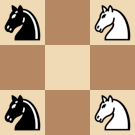
\includegraphics[height=2cm]{guarinis-problem.png}  
\end{center}

\vspace{0.2cm}

\noindent In one step, a knight can move two squares horizontally and one vertically, 
or two vertically and one horizontally. The white knights and the black knights wish to exchange
places.

\begin{subprob}
 \item Model this problem with a simple graph.
 \item From the graph representation, conclude that there is or isn't a way for the white knights and the black
 knights to exchange places. 
\end{subprob} 
\end{problem}





\section{Graphs ({\bf max 40}) }

\begin{problem}
 \item (5 points) For every $k$-regular graph is there a $(k+1)$-regular graph that contains the $k$-regular graph as a subgraph?
\end{problem}

\begin{problem}
 \item (5 points) Prove that if a graph $G$ has exactly two vertices $u$ and $v$ of odd degree, then $G$ has a $u,v$-path.
\end{problem}


\begin{problem}
 \item (10 points) 
 The \emph{complement} $\bar G$ of a simple graph $G$ is the graph with the same vertices
  as $G$ that has an edge between vertices $u$ and $v$ if and only if
  there is no edge between $u$ and $v$ in $G$.
  \begin{subprob}
    \item If $G$ is not connected,  what can you say about the connectivity
    of $\bar G$?
    \item Give an example of a graph $G$ such that both $G$ and $\bar G$ are connected.
  \end{subprob}
\end{problem}
 
 

\begin{problem}
 \item (10 points) 
 Is there a simple graph on $n\ge 2$ vertices such that the vertices all have distinct degrees? Is there a (general) graph with this property? 
\end{problem}


\begin{problem} 
 \item (10 points) 
 Show that every simple graph with average degree $\bar d$ contains a subgraph of minimal degree at least $\bar d/2$.
\end{problem}


\begin{problem}
 \item (10 points) A \textit{bridge} is an edge whose removal from the graph increases the number of connected components.
  Show that a simple $r$-regular bipartite graph with $r \ge 2$ does not have a bridge.
\end{problem}


\begin{problem} 
 \item (5 points) 
 For $r,s\in \NN$ with $2\le r\le s$, show that complete graphs $K_r$ and $K_s$ together have fewer edges than $K_{r-1}$ and $K_{s+1}$ together:
\[
|E(K_r)| + |E(K_s)| < |E(K_{r-1})| + |E(K_{s+1})|.
\]
Use this to show that a simple graph $G$ with $n$ vertices and $k$ components has the maximum number of edges when one component is $K_{n-k+1}$ and the remaining $k-1$ are each a single vertex. 
\end{problem}




\section{Digraphs ({\bf max 17})}

\begin{problem}
 \item (5 points) 
 For $n \ge 3$, let $\mathcal{C}(n)$ be the collection of digraphs $\vec{G}$ with
 $V(\vec{G}) = \{u_1, \dots, u_n\}$ that satisfy the following two conditions:
 \begin{itemize}
  \item The underlying graph of each digraph in $\mathcal{C}(n)$ is the cycle $C_n$.
  \item No digraph in $\mathcal{C}(n)$ is a directed cycle.
 \end{itemize}
\noindent  What is the cardinality of $\mathcal{C}(n)$?
\end{problem}



\begin{problem}
 \item (8 points)
 In a certain country, there is a single one-way street between every two cities. Show that there is a  city from which you can travel to any other city (by car and without traffic violations). \small{Hint: Use induction.}
\end{problem}



\begin{problem}
 \item (8 points)
Show that every connected simple graph with an even number of edges has an orientation in which every vertex $v$ has even out-degree $d^+(v)$.
\end{problem}



\section{Graph Minors ({\bf max 8}) }

\begin{problem}
 \item (5 points) Show that $K_n$ is always a contraction of $K_{n+1}$. Is $K_{n,n}$ always a contraction of $K_{n+1, n+1}$?
\end{problem}

\begin{problem}
 \item (5 points)
 Show that for every $n \in \mathbb{N}$, $K_n$ is a contraction of $K_{n,n}$. 
\end{problem}





\section{Trees ({\bf max 13})}

\begin{problem}
 \item (10 points)
 Let $T$ be a graph. Show that these assertions are equivalent:

  \begin{subprob}
  \item $T$ is a tree;
  \item Between any two vertices of $T$ there is a unique path;
  \item $T$ is maximally connected, that is, $T$ is connected, but removing any edge disconnects it;
  \item $T$ is maximally acyclic, that is, $T$ is acyclic, but adding an edge between any pair of non-adjacent vertices creates a cycle.
  \end{subprob}
\end{problem}


\begin{problem}
 \item (5 points) Draw the eleven unlabeled trees on seven vertices.
\end{problem}

 
\end{document}
